\chapter{Lezione 8-03-2024}
\section{Introduzione}
\begin{definizione}
    Possiamo definire un agente intelligente come un sistema che percepisce
    l'ambiente e agisce su di esso.
\end{definizione}

Possiamo definire l'intelligenza artificiale attraverso lo studio di agenti,
stiamo \textbf{Agentification of AI}, ovvero la consideriamo come un singolo
agente che risolve i problemi, adottando diverse strategie.

\section{Agenti}
Il termine \textbf{agente} viene definito in diversi modi da diversi autori,
vogliamo ora riportare alcune definizioni di agente:
\begin{definizione}[Russel e Norvig]
    Un \textbf{agente} è qualcosa che percepisce l'ambiente attraverso sensori e
    agisce su di esso attraverso attuatori.
\end{definizione}
\begin{figure}
    \centering
    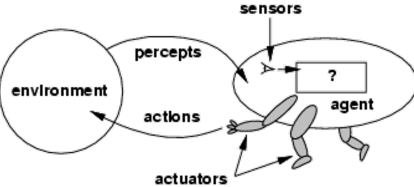
\includegraphics[width=0.5\textwidth]{./1_anno/SCMS/img/AgenteEAmbiente.png}
    \caption{Schema di un agente}
    \label{fig:agenti}
\end{figure}
Di un agente possiamo definire la \textbf{funzione agente} che mappa la storia
delle percezioni in una azione, ovvero:
\begin{equation}
    f: P^* \rightarrow A
\end{equation}
dove $P^*$ è l'insieme delle parti delle sequenze di percezioni e $A$ è l'insieme
delle azioni.

Oltre a ciò possiamo definire il \textbf{programma} dell'agente che viene
eseguito sulla sua \textbf{architettura} fisica per svolgere la funzione agente.
\begin{center}
    Agent = Program + Architecture
\end{center}

Col passare del tempo si è passati da un singolo agente che calcola la soluzione
a un sistema di entità che collaborano per risolvere un problema.
\begin{definizione}
    Un sistema è un gruppo di elementi che formano un insieme che collabora per
    raggiungere un obiettivo comune. Questo ci dice che un sistema è qualcosa in
    più di un singolo insieme di elementi, in quanto è presente un organizzazione
    tra le parti che lo compongono.
\end{definizione}

Prima abbiamo accennato a un sistema di entità che collaborano per risolvere un
problema, questo sistema può essere distribuito. Vogliamo ora capire cosa
può essere distribuito:
\begin{itemize}
    \item Possiamo avere che la soluzione di un problema è distribuita, ovvero
          la soluzione del problema richiede capacità che appartengono a più
          entità.
    \item Possiamo avere un problema distribuito in cui le entità che risolvono
          il problema sono distribuite oppure centralizzate. Come esempio di
          problema distribuito possiamo pensare a un problema di coordinamento
          i robot che lavorano in un magazzino.
\end{itemize}

Un aspetto critico degli approcci basati su sistemi multi agente è dovuto al
fatto che le azioni svolte da un agente non sono solamente interne a esso, ma
possono influenzare l'ambiente e quindi anche gli altri agenti.
\section{Architettura degli agenti}
Una prima classificazione degli agenti è quella di Genesereth la quale si basa
sul fatto che gli agenti possono essere classificati in base alle loro capacità
interne e alle risorse a loro disposizione. Questa prima classificazione
distingue gli agenti in:
\begin{itemize}
    \item \textbf{Tropistic}
    \item \textbf{Hysteretic}
    \item \textbf{Knowledgw-based}
\end{itemize}
\begin{nota}
    Questa analisi è stata effettuata considerando un singolo agente, ma
    possiamo estendere questa analisi a sistemi multi agente.
\end{nota}
\subsection{Tropistic Agents}
In questa classe gli agenti sono definiti attraverso una tupla composta da 6
elementi:
\begin{equation*}
    \langle E, P, A, \text{see}, \text{do}, \text{action} \rangle
\end{equation*}
dove:
\begin{itemize}
    \item $E$ è l'insieme degli stati dell'ambiente.
    \item $P$ è l'insieme delle percezioni, è una partizione di $E$.
    \item $A$ è l'insieme delle azioni.
    \item \textbf{see} è una funzione che mappa $E$ in $P$ e rappresenta quello
          che l'agente vede dell'ambiente.
    \item \textbf{action} è una funzione che mappa $P$ in $A$ è una funzione che
          seleziona l'azione che l'agente deve svolgere in base a una determinata
          percezione. È importante notare che abbiamo perso il fatto che il
          dominio non è l'insieme potenza delle percezioni.
    \item \textbf{do} è una funzione che mappa $A \times E$ in $E$ e rappresenta
          l'effetto di un'azione sull'ambiente.
\end{itemize}

In questa classe gli agenti osservano l'ambiente, scelgono l'azione appropriata
e la eseguono.
\subsection{Hysteretic Agents}
Gli agenti hysteretic sono definiti attraverso una tupla composta da 9 elementi:
\begin{equation*}
    \langle I, E, P, A, i_0, \text{see}, \text{internal,} \text{do}, \text{action} \rangle
\end{equation*}
dove:
\begin{itemize}
    \item $I$ è l'insieme degli stati interni.
    \item $E$ è l'insieme degli stati dell'ambiente.
    \item $P$ è l'insieme delle percezioni, è una partizione di $E$.
    \item $A$ è l'insieme delle azioni.
    \item $i_0$ è lo stato iniziale dell'agente.
    \item \textbf{see} è una funzione che mappa $E$ in $P$ e rappresenta quello
          che l'agente vede dell'ambiente.
    \item \textbf{internal} è una funzione che mappa $P \times I$ in $I$ e
          rappresenta l'effetto di una percezione sullo stato interno dell'agente.
    \item \textbf{do} è una funzione che mappa $A \times E$ in $E$ e rappresenta
          l'effetto di un'azione sull'ambiente.
    \item \textbf{action} è una funzione che mappa $P \times I$ in $A$ è una funzione
          che seleziona l'azione che l'agente deve svolgere in base a una determinata
          percezione e stato interno.
\end{itemize}
In questa classe gli agenti osservano l'ambiente, aggiornano il loro stato interno
e scelgono l'azione appropriata e la eseguono.
\subsection{Knowledge-based Agents}
Gli agenti knowledge-based sono definiti attraverso una tupla composta da 9 elementi:
\begin{equation*}
    \langle D, E, P, A, d_0, \text{see}, \text{database}, \text{do}, \text{action} \rangle
\end{equation*}
dove:
\begin{itemize}
    \item $D$ è l'insieme delle conoscenze dell'agente.
    \item $E$ è l'insieme degli stati dell'ambiente.
    \item $P$ è l'insieme delle percezioni, è una partizione di $E$.
    \item $A$ è l'insieme delle azioni.
    \item $d_0$ è lo stato iniziale del database dell'agente.
    \item \textbf{see} è una funzione che mappa $E$ in $P$ e rappresenta quello
          che l'agente vede dell'ambiente.
    \item \textbf{database} è una funzione che mappa $P \times D$ in $D$ e
          rappresenta l'effetto di una percezione sul database dell'agente.
    \item \textbf{do} è una funzione che mappa $A \times E$ in $E$ e rappresenta
          l'effetto di un'azione sull'ambiente.
    \item \textbf{action} è una funzione che mappa $P \times D$ in $A$ è una funzione
          che seleziona l'azione che l'agente deve svolgere in base a una determinata
          percezione e stato interno.
\end{itemize}
In questa classe gli agenti osservano l'ambiente, aggiornano il loro database
e scelgono l'azione da svolgere in in base a un ragionamento sulle conoscenze
possedute e infine eseguono l'azione.
\section{Russell e Norvig}
Una differente classificazione degli agenti è quella Russell e Norvig, la quale
classifica gli agenti in base alla loro architettura interna. Questa classificazione
distingue gli agenti in:
\begin{itemize}
    \item \textbf{Simple reflex agents}
          \begin{figure}[!ht]
              \centering
              \includegraphics[width=0.5\textwidth]{./1_anno/SCMS/img/Agenti/SimpleReflexAgent.png}
              \caption{Schema di un agente}
              \label{fig:simpleReflex}
          \end{figure}
    \item \textbf{Model-based reflex agents}
          \begin{figure}
              \centering
              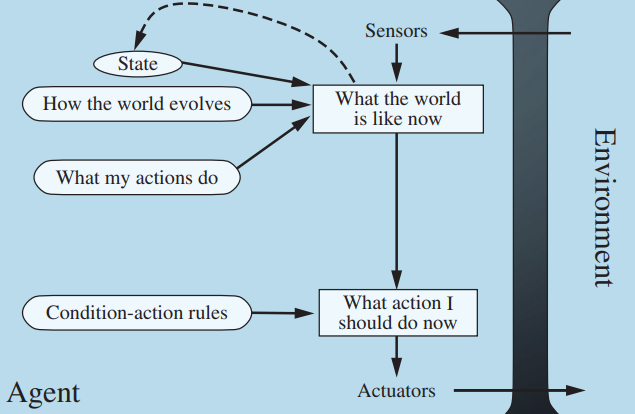
\includegraphics[width=0.5\textwidth]{./1_anno/SCMS/img/Agenti/ModelBasedReflexAgent.png}
              \caption{Schema di un agente}
              \label{fig:ModelReflex}>
          \end{figure}
    \item \textbf{Goal-based agents}: l'agente deve sapere quali sono le
          situazioni desiderate e quali azioni devono essere svolte per raggiungere
          tali situazioni. Possono essere più flessibili dato che la conoscenza
          è rappresentata in modo esplicito e può essere manipolata.
          \begin{figure}
              \centering
              \includegraphics[width=0.5\textwidth]{./1_anno/SCMS/img/Agenti/GoalBasedAgent.png}
              \caption{Schema di un agente}
              \label{fig:GoalBased}
          \end{figure}
    \item \textbf{Utility-based agents}: in questo caso uno stesso obiettivo può
          essere raggiunto in modi diversi. Viene definita una funzione di utilità che
          che descrive il grado di soddisfazione dell'agente in base alla situazione
          in cui si trova.
          \begin{figure}
              \centering
              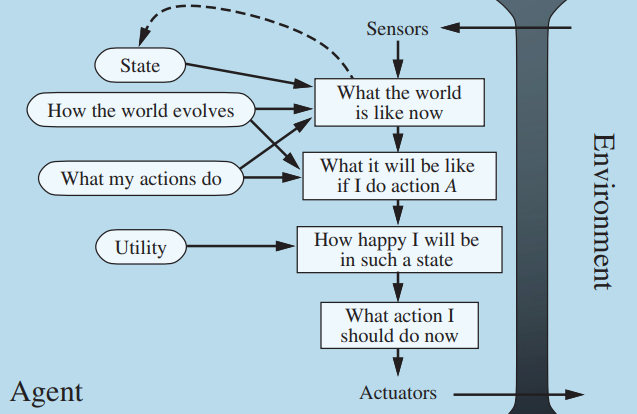
\includegraphics[width=0.5\textwidth]{./1_anno/SCMS/img/Agenti/UtilityBasedAgent.png}
              \caption{Schema di un agente}
              \label{fig:UtilityBased}
          \end{figure}
\end{itemize}

La prima classe di questa classificazione corrisponde alla classe degli agenti
tropistic, la seconda classe corrisponde alla classe degli agenti hysteretic. Le
altre due classi sono invece una specializzazione della classe knowledge-based.